\documentclass[12pt,a4paper]{article}
\usepackage[UTF8]{ctex}
\usepackage{amsmath,amssymb}
\usepackage{graphicx}
\usepackage{booktabs}
\usepackage{float}
\usepackage{geometry}
\usepackage{listings}
\usepackage{xcolor}

\geometry{a4paper,left=2.5cm,right=2.5cm,top=2.5cm,bottom=2.5cm}

\title{一维线性输运方程数值解法实验报告}
\author{刘行 PB22000150}
\date{\today}

\begin{document}
    \maketitle

    \section{问题描述}
        本实验研究一维线性输运方程的数值求解方法. 该方程在流体力学, 气象学等领域具有广泛应用, 其形式为:
        \begin{equation}
            \frac{\partial u}{\partial t} + a \frac{\partial u}{\partial x} = 0
        \end{equation}
        其中$a$为波速. 在本实验中, 我们考虑 $a = -1$ 的情况, 即方程变为 $u_{t} = u_{x}$. 初始条件给定为 $u\left(x,0\right) = \sin\left(2\pi x\right)$, 边界条件采用周期性边界条件, 计算域为 $\left[0,1\right]$, 终止时间 $T = 0.3$.

        该问题的解析解可以通过特征线法求得. 由于方程描述的是波的传播, 解沿特征线$x - t = C$保持不变, 因此解析解为$u(x,T) = \sin\left(2\pi\left(x+T\right)\right)$. 通过比较数值解与解析解, 我们可以评估不同数值格式的精度和稳定性.

        线性输运方程虽然形式简单, 但能够很好地检验数值格式的基本性质, 如稳定性, 精度和耗散性等. 特别是对于对流占优问题, 数值格式的选择对计算结果影响显著. 本实验旨在通过该模型方程, 深入理解数值方法的基本特性.

    \section{数值方法}
        本实验采用迎风格式 (Upwind Scheme) 离散输运方程. 对于方程 $u_t = u_x$, 迎风格式的离散形式为:
        \begin{equation}
            u_{j}^{n+1} = u_{j}^{n} + \frac{\Delta t}{\Delta x}\left(u_{j+1}^{n} - u_{j}^{n}\right)
        \end{equation}
        其中 $\Delta t$ 为时间步长, $\Delta x$ 为空间步长, $u_{j}^{n}$ 表示第 $n$ 时间层, 第 $j$ 空间点的数值解.

        迎风格式的稳定性由CFL (Courant-Friedrichs-Lewy) 条件决定. 对于线性输运方程, CFL条件要求:
        \begin{equation}
            \nu = \left\lvert\frac{\Delta t}{\Delta x}\right\rvert \leq 1
        \end{equation}
        其中$\nu$称为 CFL 数. 当 CFL 数小于等于 1 时, 数值格式稳定; 当 CFL 数大于 1 时, 数值格式不稳定.

        迎风格式的稳定性分析可以通过 Von Neumann 稳定性分析方法进行. 将傅里叶模式 $u_j^{n} = \xi^{n} e^{ikj\Delta x}$ 代入离散格式, 可得放大因子:
        \begin{equation}
            \xi\left(k\right) = 1 + \nu\left(e^{ik\Delta x} - 1\right)
        \end{equation}
        稳定性要求对所有波数 $k$ 满足 $\left\lvert\xi\left(k\right)\right\rvert \leq 1$, 这导出 $\nu \leq 1$ 的条件.

        迎风格式具有一阶精度, 且具有数值耗散特性. 数值耗散会使解的高频分量衰减, 导致数值解比精确解更加光滑. 这种耗散性在某些情况下是有益的, 可以抑制数值振荡, 但也会降低解的精度.

    \section{数值实验结果}
        \subsection{初始实验结果}
            初始实验设置了两种不同的时间步长, 空间离散点数固定为$J=50$. 实验结果如下:

            当 $\Delta t = 0.01$ ($N=30$) 时, CFL 数为 0.5, 满足稳定性条件, 误差为:
            \begin{verbatim}
                err_2 = 4.100489e-02, err_inf = 5.742160e-02
            \end{verbatim}

            当 $\Delta t = 0.03$ ($N=10$) 时, CFL 数为 1.5, 违反稳定性条件, 误差为:
            \begin{verbatim}
                err_2 = 4.334540e-02, err_inf = 6.075086e-02
            \end{verbatim}

            对应的数值解与精确解的比较如图 \ref{fig:result_001} 和图 \ref{fig:result_003} 所示.

            \begin{figure}[H]
                \centering
                \begin{minipage}{0.45\textwidth}
                    \centering
                    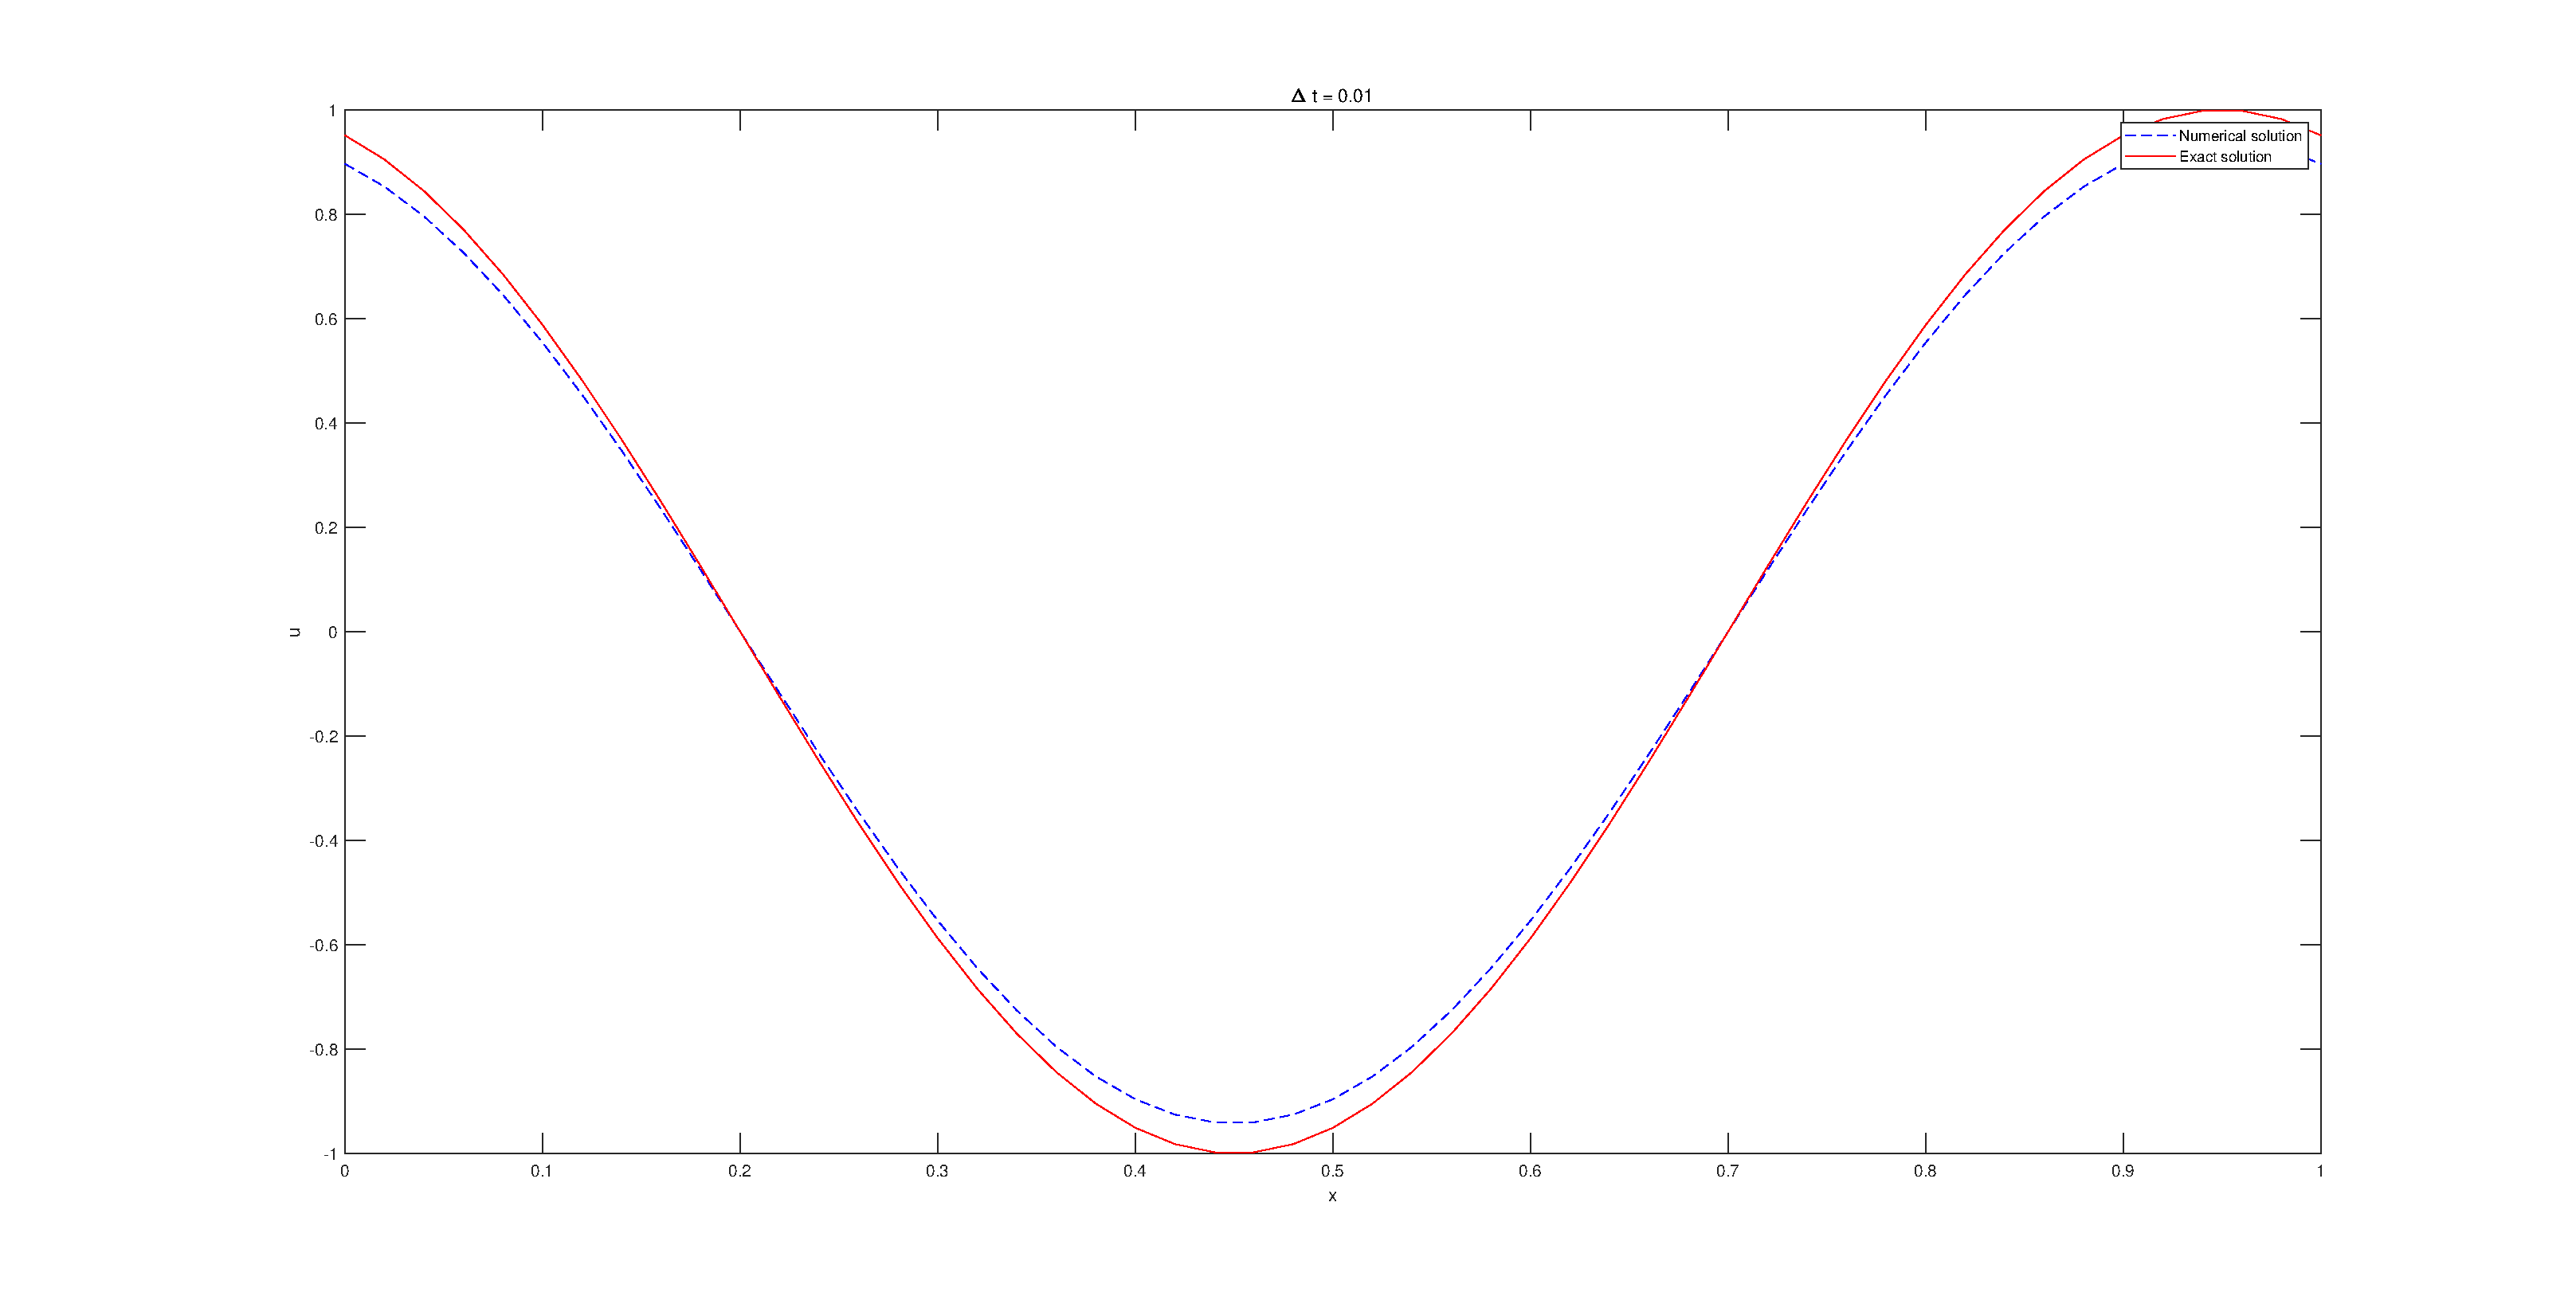
\includegraphics[width=\linewidth]{fig/result_001.eps}
                    \caption{$\Delta t = 0.01$ 时数值解与精确解比较}
                    \label{fig:result_001}
                \end{minipage}
                \hfill
                \begin{minipage}{0.45\textwidth}
                    \centering
                    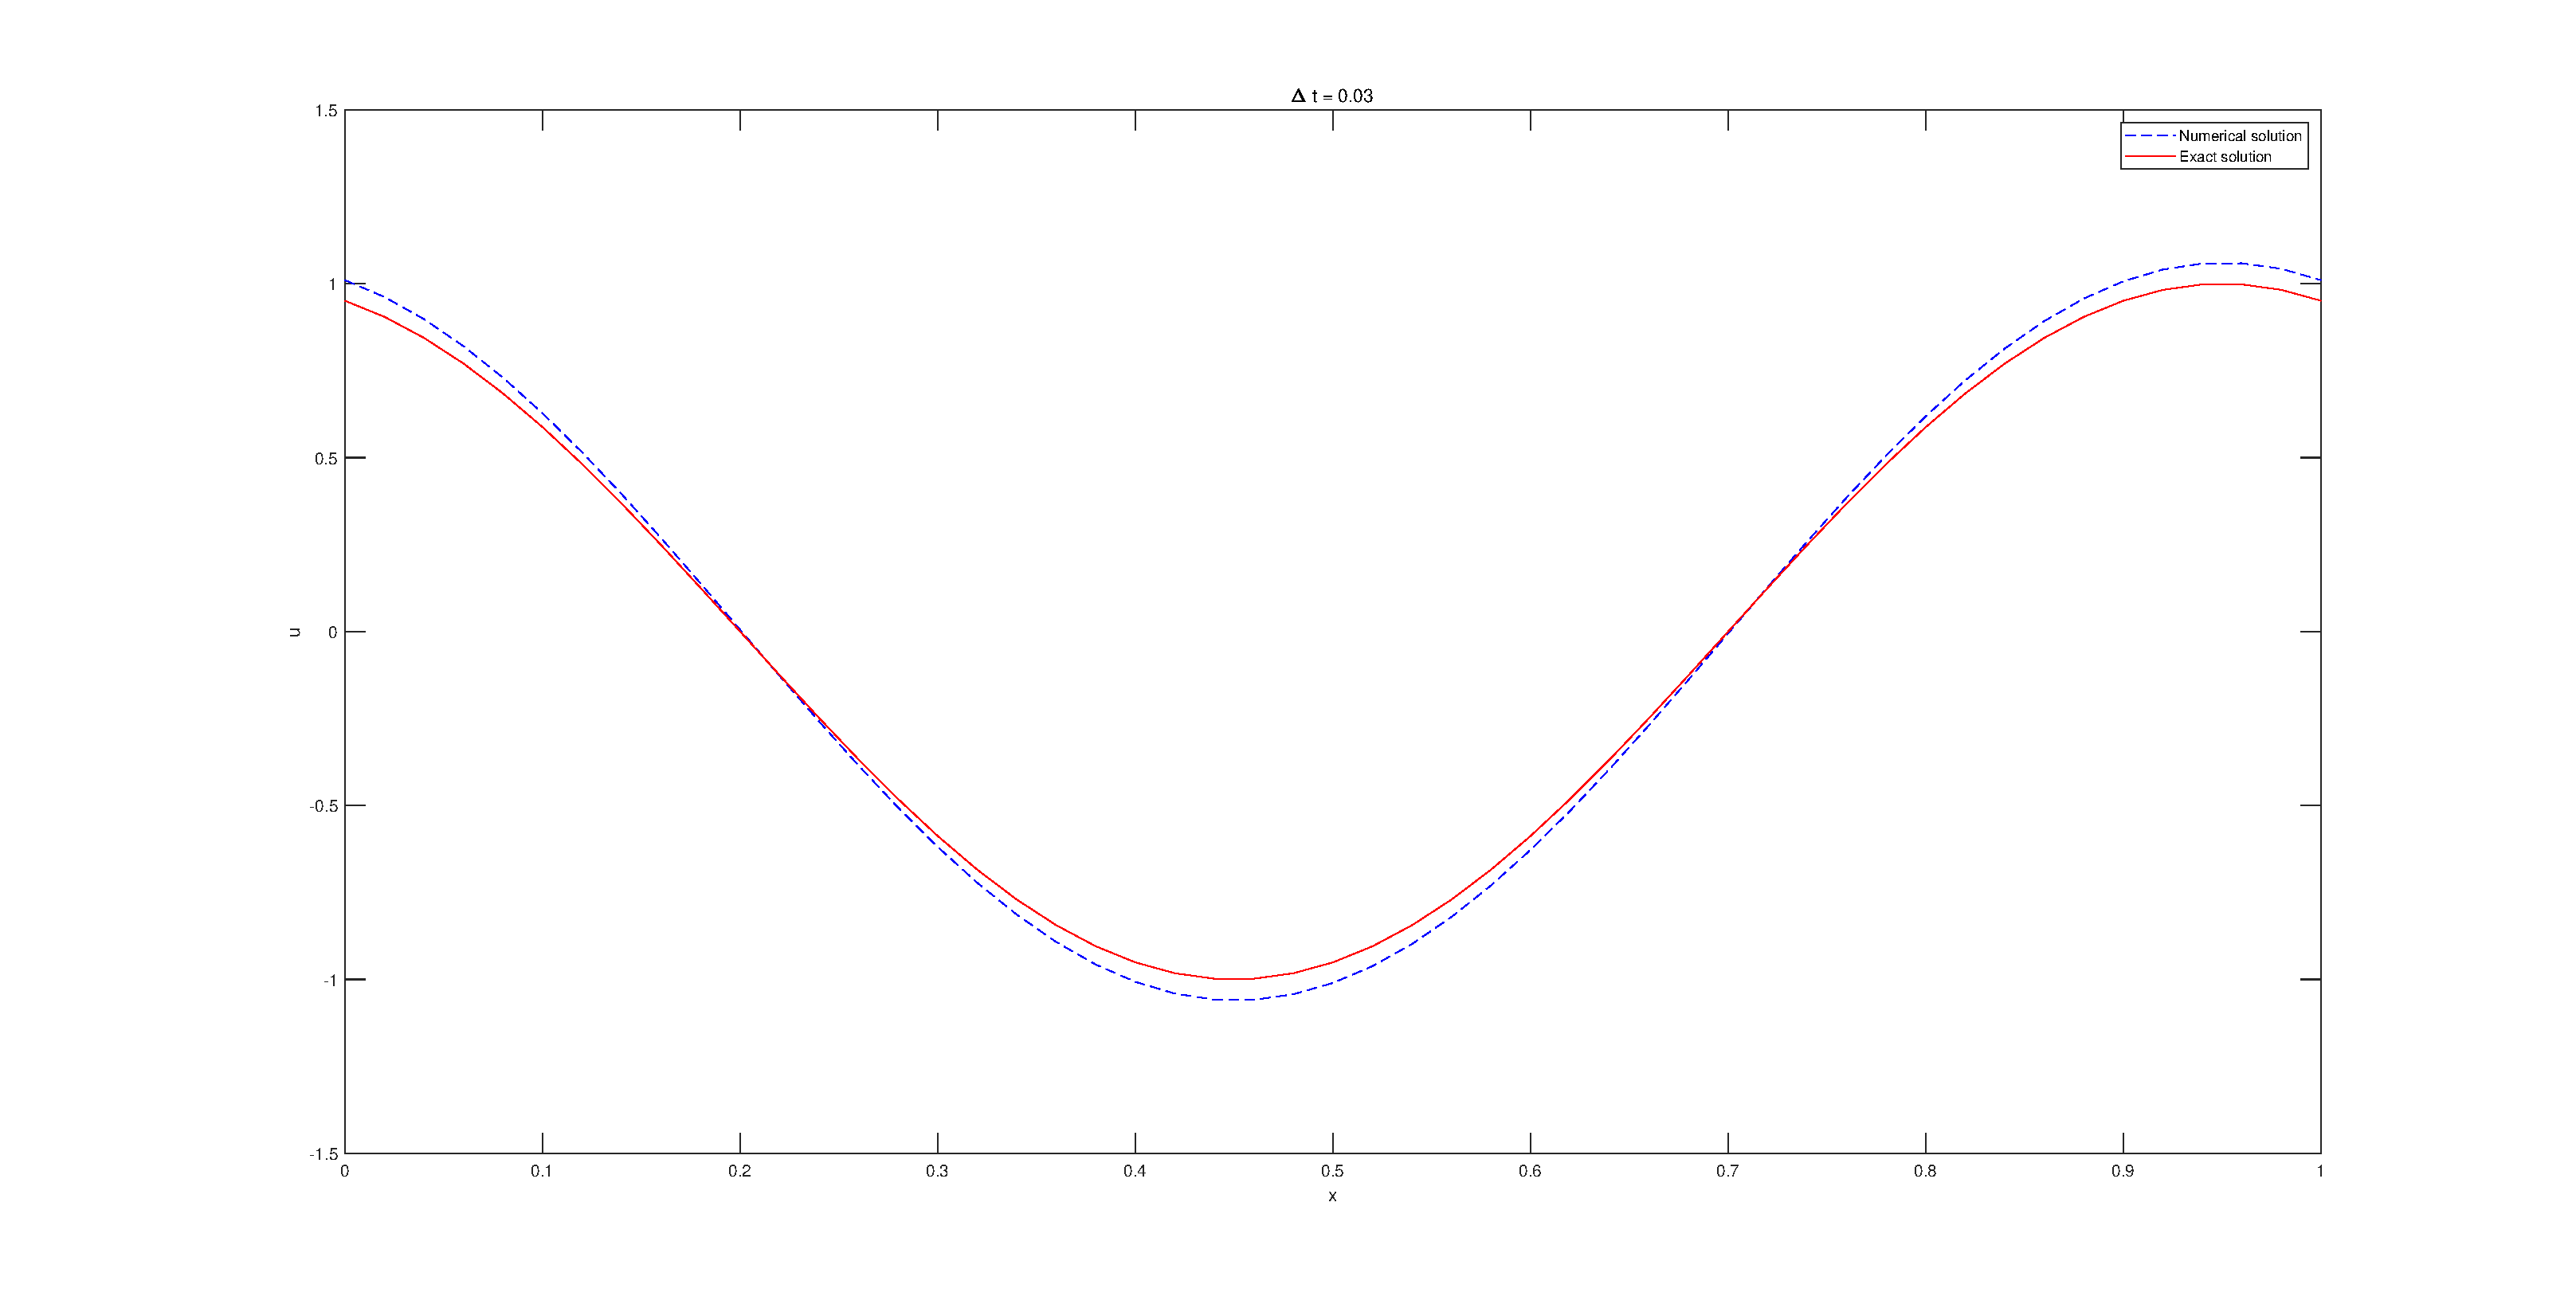
\includegraphics[width=\linewidth]{fig/result_003.eps}
                    \caption{$\Delta t = 0.03$ 时数值解与精确解比较}
                    \label{fig:result_003}
                \end{minipage}
            \end{figure}

        \subsection{理论与实验的不一致性分析}
            理论上, 当 CFL 数大于 1 时, 迎风格式应该不稳定, 数值解应该发散. 但初始实验结果显示, 即使 CFL 数为 1.5, 数值解也没有明显发散, 只是精度略有下降.

            这种理论与实验的不一致性源于计算时间不够长, 数值不稳定的增长尚未充分发展. 在 \texttt{src/test.m} 中的进一步测试表明, 当增加计算时间或细化网格时, 不稳定性会变得更加明显.

            数值不稳定性的发展需要一定的时间步数才能显现. 对于线性问题, 不稳定模式的增长通常是指数形式的, 但在初始阶段增长可能很缓慢. 此外, 数值耗散也会在一定程度上抑制不稳定性的发展.

            当空间网格进一步细化时 (如$J=300$), 可以观察到 CFL 数大于 1 时误差急剧增大, 如图 \ref{fig:result_compare} 所示, 且 $L_{\infty}$ 误差达到 $9.18\times10^1$, 这符合理论预期的不稳定行为.

            \begin{figure}[H]
                \centering
                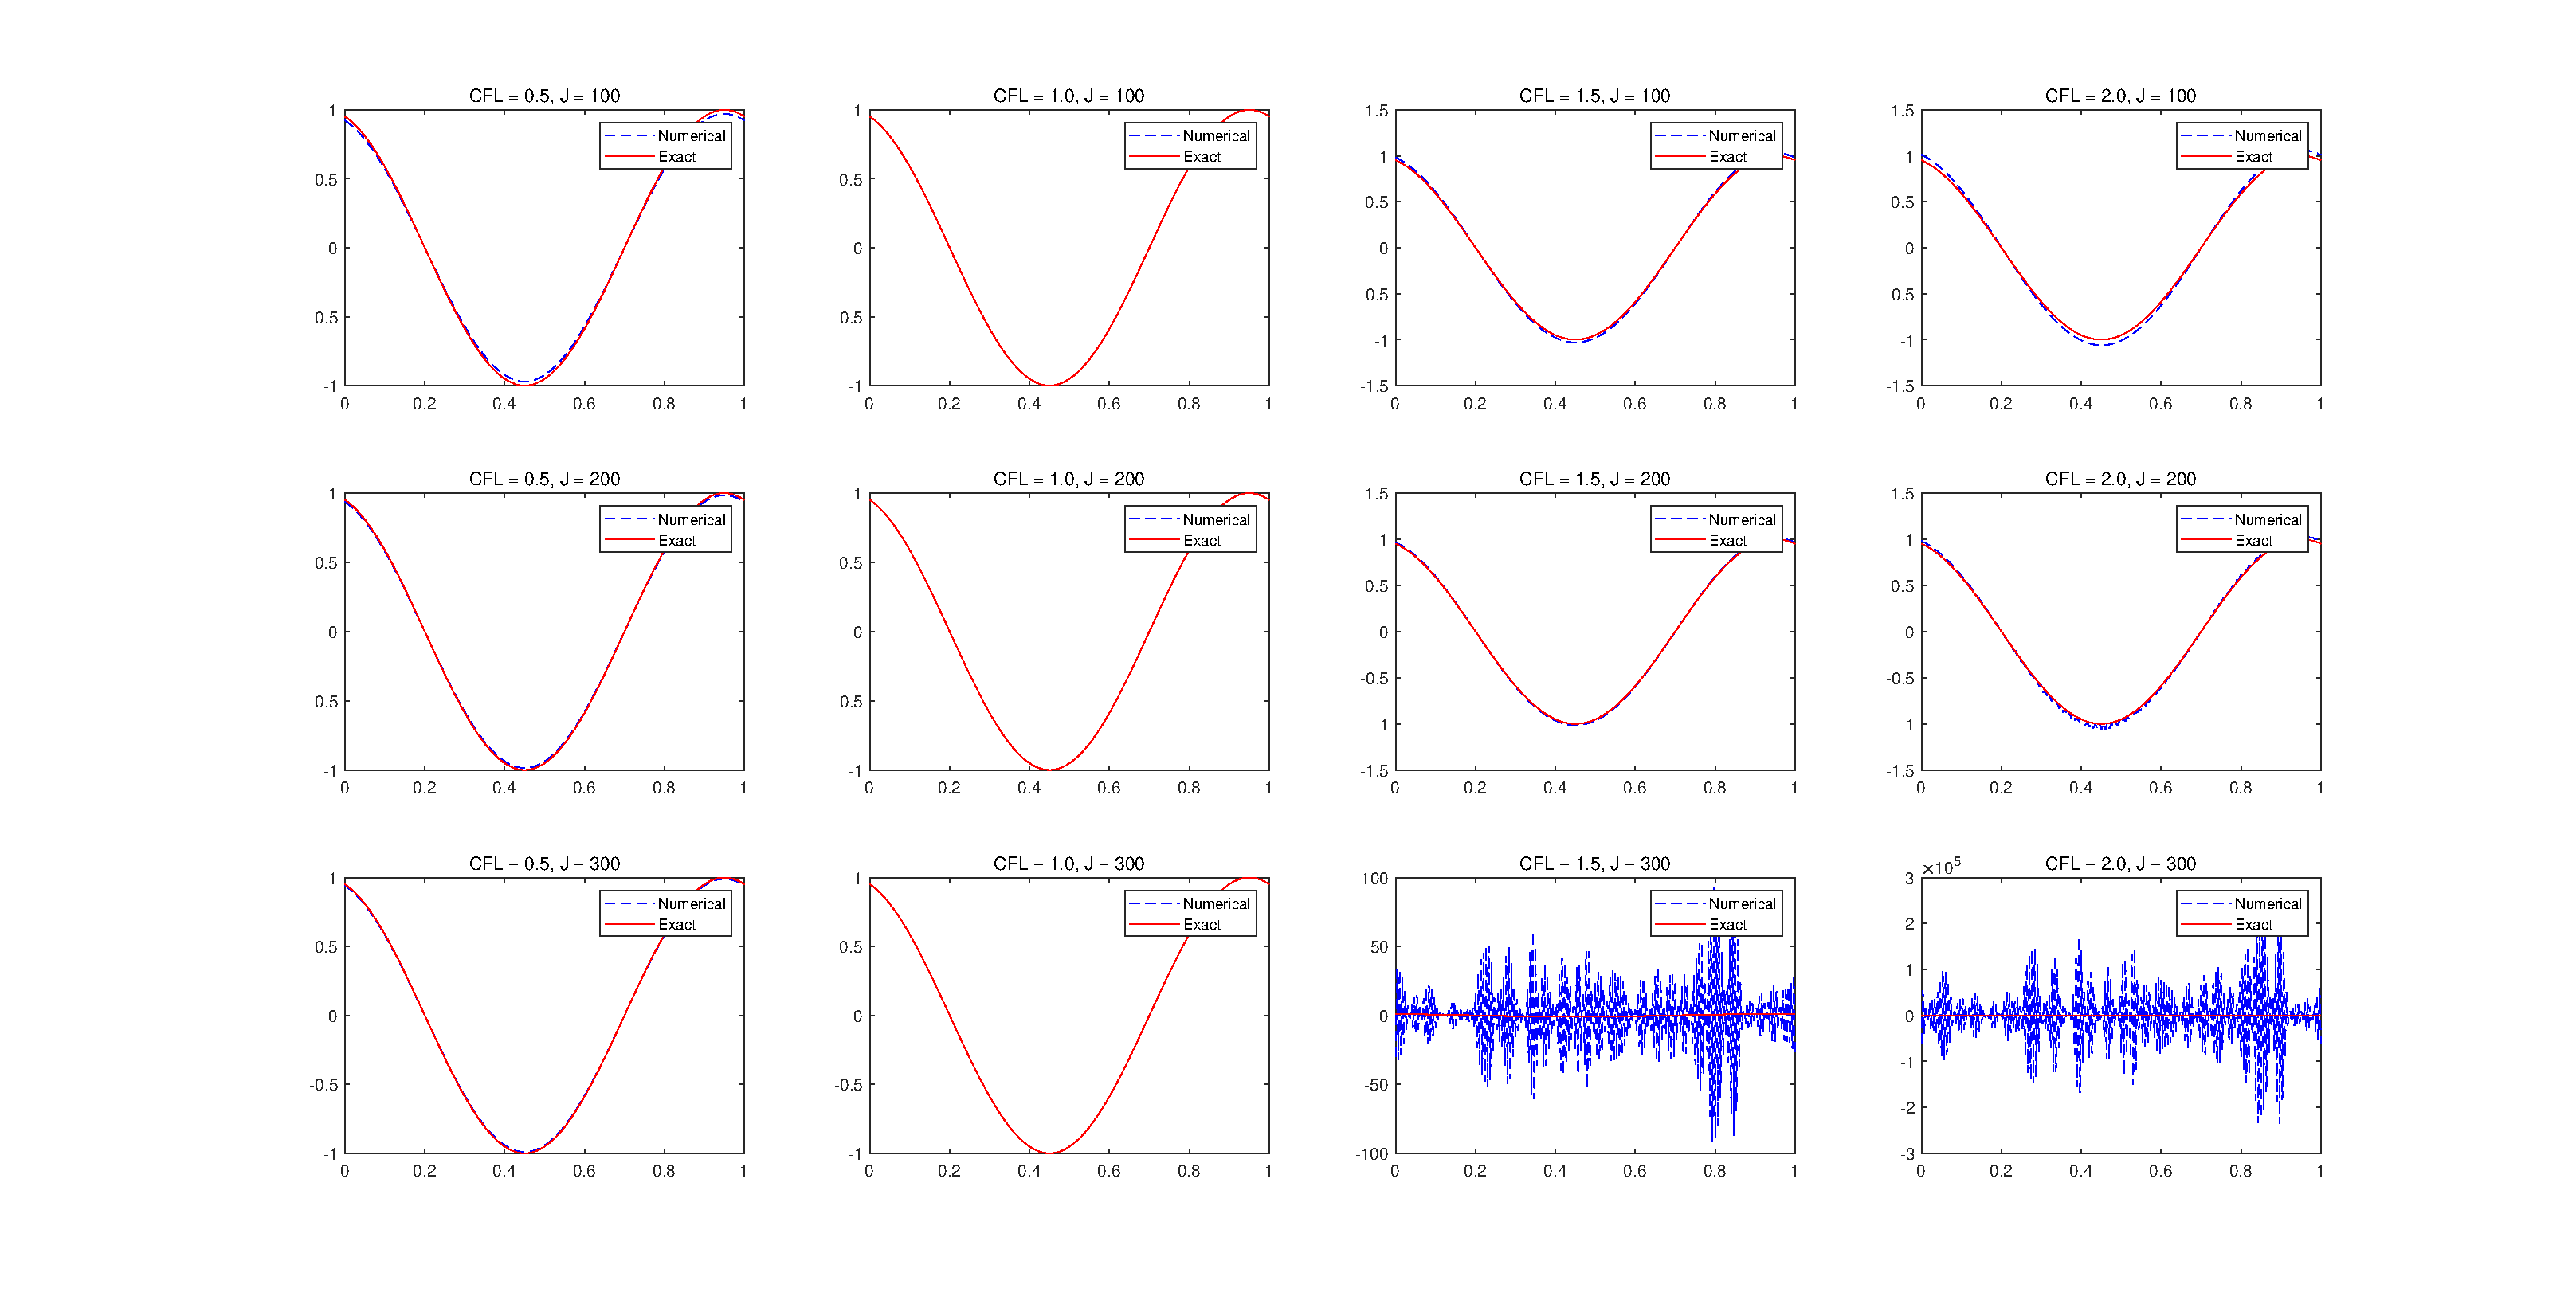
\includegraphics[width=\textwidth]{fig/result_compare.eps}
                \caption{不同空间网格及 CFL 数下数值解与精确解比较}
                \label{fig:result_compare}
            \end{figure}

    \section{结论}
        通过本实验, 我们得到以下主要结论:

        首先, 迎风格式对于线性输运方程在CFL数小于等于1时是稳定的, 这符合理论分析结果. 数值实验验证了CFL条件的重要性, 它是保证数值方法稳定性的必要条件.

        其次, 数值不稳定的发展需要足够的计算时间才能显现. 短时间计算可能无法充分暴露数值方法的不稳定性, 这在实践中需要特别注意. 工程设计中的长时间模拟必须严格满足稳定性条件.

        第三, 迎风格式具有数值耗散特性, 这在一定程度上可以抑制数值振荡, 但也会降低解的精度. 在实际应用中, 需要根据具体问题权衡数值耗散的利弊.

        最后, 本实验强调了理论分析与数值实验相结合的重要性. 单纯依靠理论或实验都可能得到片面的结论, 只有将两者结合才能深入理解数值方法的特性.

        这些结论对于计算流体力学中的数值方法选择具有指导意义, 提醒我们在实际计算中必须充分考虑数值方法的稳定性, 精度和计算效率之间的平衡.

\end{document}
